%!TEX root = ../DSGEnotes.tex
\chapter{映射法}

\section{简介}
映射法(projection methods)\index{projection method \dotfill 映射法},又称加权残差法(weighted residual methods)\index{weighted residual methods \dotfill 加权残差法}。利用映射法求解DSGE模型是指,找到一组合适的系数向量$\theta = \left\{
\theta_0, \theta_1, \ldots, \theta_j \right\}$和一组基方程(basis function) \index{basis function \dotfill 基方程} $\Psi_i(\bm{x})$ 后,假定$\theta$和$\Psi_i(x)$呈现线性组合方程$d^{j}(\bm{x}|\theta)$
\begin{equation}
  \label{eq:pj-linear-combination-theta-psi}
  d^{j}(\bm{x}|\theta) = \sum_{i=0}^{j}\theta_{i} \Psi_i(\bm{x}),
\end{equation}
进而用$d^j(\bm{x}|\theta)$来近似$d(\bm{x})$,进而求解$\mathcal{H}(d) = 0$,即是说,定义一个残差方程 (residual function) \index{residual function (projection method) \index{残差方程(映射法)}}  $R(\bm{x}|\theta) = \mathcal{H}\left( d^j(\bm{x}|\theta) \right)$,通过$\theta$系数的选取实现残差方程的最小化
\begin{equation}
  \label{eq:pj-residual-function-def}
  \min_{\{\theta\}} \left| R(\bm{x}|\theta) \right|,
\end{equation}
这称为对$\mathcal{H}$做$\Psi$的映射,以求最佳系数$\theta$。

在操作层面上,这意味着首先如\eqref{eq:pj-linear-combination-theta-psi}, 选取某种恰当的基$\left\{ \Psi_i (\bm{x})\right\}_{i=0}^{\infty}$,用基与系数内积并求和的方法构建$d(\bm{x} | \theta)$;进而如\eqref{eq:pj-residual-function-def},对$\mathcal{H}$做$\Psi$的映射,求得$\theta$。就这两个环节来说,显然,选取不同形式的基和映射算法的组合,会出现不同的映射法,在不同的文献中,有时也会给它们以一些专有的称呼,以与其他映射法相区分。

经济学家很早就将映射理论应用到经验研究中去了,进入20世纪90年代后,映射法逐渐成为一种成熟的宏观经济学研究方法,主要归功于\cite{Judd:1992vv,Gaspar:1997we,Judd:1998uy}的贡献\footnote{与扰动法相比,映射法的思路更为现代,但在自然科学、工程学研究中也有许多年的悠久历史了。映射法的前身之一光谱法(spectral methods)至少可上溯至\cite{Lanczos:1938hy},另一个前身有限元法(finite elements methods, FEM)来自于波音工程师\cite{Clough:1960wq}的开创性工作;关于有限元法的早期发展可见\cite{Clough:1999uo}。}。

大致说来,映射法比扰动法更易于描述,但算法实现上则较为困难。下面是一个映射法的基本算法描述:
\begin{algorithm}[映射法的基本算法] 可简述如下:
  \begin{enumerate}
    \item 对于正整数$j < \infty$,定义$j+1$个线性不相关方程$\Psi_i:\Omega \mapsto \mathbb{R}, \quad i=0,1,\ldots,j$。则$\left\{\Psi_{i}\right\}_{0}^{j} = \psi_0, \psi_1, \ldots, \psi_j$称为基方程,是与状态变量向量$\bm{x}$有关的方程。

    \item 对于正整数$m < \infty$ ($m$是方程系统$d(\bm{x})$所映射的维度),系数向量$\theta^{l} = \left[  \theta_0^{l}, \theta_1^{l}, \ldots, \theta_j^{l} \right], \quad l = 1,2,\ldots,m$。将$m$组系数向量合并组成系数矩阵
    \begin{equation*}
      \underset{ \left\{ m \times (j+1) \right\}}{\theta} = \begin{pmatrix}
      \theta^1 \\
      \theta^2 \\
      \vdots \\
      \theta^m \\
    \end{pmatrix}
    = \begin{pmatrix}
    \theta_0^{1}& \theta_1^{1}& \ldots & \theta_j^{1}  \\
    \theta_0^{2}& \theta_1^{2}& \ldots & \theta_j^{2}  \\
    \vdots & \vdots & \ddots & \vdots\\
    \theta_0^{m}& \theta_1^{m}& \ldots & \theta_j^{m}
    \end{pmatrix}.
    \end{equation*}
    \item 定义内积求和方程
    \begin{equation*}
      d^{l,j}(\cdot | \theta^{l}) = \sum_{i=0}^{j} \phi_{i}^{l} \psi_i(\cdot),
    \end{equation*}
    则对应地我们有
    \begin{equation*}
      \underset{ \left\{ m \times 1 \right\} } {d^{j}(\cdot | \theta)}
      = \begin{pmatrix}
      d^{1, j}(\cdot | \theta^{1})\\
      d^{2, j}(\cdot | \theta^{2})\\
      \vdots \\
      d^{m, j}(\cdot | \theta^{m})
      \end{pmatrix}.
    \end{equation*}
    \item 将$d^{j}(\cdot | \theta)$作为$d(\cdot)$的近似,代入$\mathcal{H}(\cdot) = 0$,构建残差方程
    \begin{equation*}
      R(\cdot | \theta) = \mathcal{H} \left(d^j ( \cdot | \theta) \right).
    \end{equation*}
    \item 定义度量方程(metric function)
    \footnote{度量方程又称距离方程 (distance function),描述集合中一对元素之间的距离。度量方程的一种,离散度量方程(discrete metric function)\index{metric function!discrete \dotfill 离散度量方程}可以表示如下\begin{equation*}
    d(x,y) =
    \begin{cases}
      0 & x=y, \\
      1 & x \neq y
    \end{cases}.
    \end{equation*}    }
    \index{metric function \dotfill 度量方程} \index{distance function \dotfill 距离方程} $\rho \left(R(\cdot | \theta), \bm{0} \right)$\todo{下文有注释,对应距离方程其实是三角方程的一种。到时把讲义内容补充到这里来。}作为目标方程,在$\theta$中找到对应的$\hat{\theta}$,满足条件
    \begin{equation*}
      \hat{\theta} = \underset{\theta \in \mathbb{R}^{m \times (j+1)}}{\arg \min} \rho \left(R(\cdot | \theta), \bm{0} \right).
    \end{equation*}
    \end{enumerate}
\end{algorithm}

\subsection{例}
\label{sec:pj-example-ncgt}
举例说明。以经典的随机内生经济增长模型为例,第\ref{sec:pta-example-ncgt}节中我们介绍了二阶扰动方法的应用。使用近似的模型,这里来介绍如何用映射法近似求解系统\footnote{第\ref{sec:pta-example-ncgt}节中的$\eta$,在这里用$\sigma$来表示。}。

第一步,改写系统。模型中的状态变量$c_t, k_{t+1}$分别表示为
\begin{equation*}
\begin{split}
    c_t = d^1 (k_t,z_t), \\
    k_{t+1} = d^{2}(k_t,z_t),
\end{split}
\end{equation*}
由此将经济系统的均衡条件(由跨期消费的欧拉等式和资源约束条件构成,即$m=2$)改写为
\begin{equation*}
\begin{split}
  &\mathcal{H}\left( d(k_t,z_t) \right) = \bm{0}, \quad \forall k_t, z_t \Rightarrow \\
  &\begin{cases}
     u'\left( d^1(k_t, z_t) \right) - \beta E_t \left\{
    u' \left( d^1 \left( d^2(k_t,z_t) ,z_{t+1}\right)\right)
    \left( \alpha \exp(\rho z_t + \sigma \varepsilon_{t+1}) \left( d^2 (k_t, z_t) \right)^{\alpha-1} + 1 - \delta \right)
    \right\} = 0, \\
     d^1(k_t,z_t) + d^2(k_t,z_t) - \exp(z_t) k_t^{\alpha} - (1-\delta) k_t = 0.
  \end{cases}
\end{split}
\end{equation*}

第二步,改写$d(\bm{x})$为$d(\bm{x}|\theta)$的形式,根据$m=2$有$\theta = \left[ \theta^1, \theta^2 \right]^{\top}$,进而定义
\begin{equation*}
\begin{split}
    &c_t = d^{1,j} \left( k_t,z_t | \theta^{1} \right) = \sum_{i=0}^{j} \theta_{i}^{1} \psi_{i}(k_t,z_t), \\
    &k_{t+1} = d^{2,j} \left(k_t,z_t | \theta^2 \right) = \sum_{i=0}^{j} \theta_{i}^{2} \psi_{i}(k_t,z_t).
\end{split}
\end{equation*}
其中$j+1$个基方程$\psi_{i}(k_t,z_t), \quad i=0,1,\ldots,j$的形式,将在下文讨论\todo{reference}。

第三步,构建残差方程$R(k_t,z_t | \theta ) = \left[ R(k_t,z_t | \theta^1 ), R(k_t,z_t | \theta^2 ) \right]^{\top} \Rightarrow$
\begin{equation*}
\begin{split}
  & R(k_t,z_t | \theta^1 ) = u'\left( \sum_{i=0}^{j} \theta_{i}^{1} \psi_{i}(k_t,z_t) \right) - \beta E_t \left\{
  u' \left( \sum_{i=0}^j \theta_i^1 \psi_i \left( \sum_{i=0}^{j} \theta_{i}^{2} \psi_{i}(k_t,z_t) , \rho z_t + \sigma \varepsilon_{t+1} \right)\right) \times \right. \\
& \qquad   \left.
 \left( \alpha \exp \left( \rho z_t + \sigma \varepsilon_{t+1} \right) \left( \sum_{i=0}^{j} \theta_{i}^{2} \psi_{i}(k_t,z_t) \right)^{\alpha-1} + 1 - \delta \right)
  \right\} , \\
&  R(k_t,z_t | \theta^2 ) = \sum_{i=0}^{j} \theta_{i}^{1} \psi_{i}(k_t,z_t) + \sum_{i=0}^{j} \theta_{i}^{2} \psi_{i}(k_t,z_t) - \exp \left( z_t \right) k_t^{\alpha} - (1-\delta) k_t.
\end{split}
\end{equation*}

第四步,构建度量方程$\rho \left(R(\cdot \theta), \bm{0} \right)$,计算
\begin{equation*}
\hat{\theta} = \underset{\theta \in \mathbb{R}^{m \times (j+1)}}{\arg \min} \rho \left(R(\cdot | \theta), \bm{0} \right),
\end{equation*}
使得相对于$\hat{\theta}$的任意$m \times (j+1)$个点$(k_l, z_l)$,都有度量$\rho =0$。为了实现这点,需要令对应的$m \times (j+1)$个残差方程最小化,换句话说,求解下述含有$m \times (j+1)$个未知数的方程系统\footnote{本讲义略过方程解的存在性与唯一性的讨论。}
\begin{equation*}
  R\left( k_l, z_l | \theta \right) = \bm{0}, \quad l \in \mathbb{R}^{m \times (j+1)}.
\end{equation*}

如上所述,采用映射法从事宏观经济学研究,关键的两点在于选择合适的基方程$\Psi(\cdot)$以及度量方程$\rho(\cdot)$,\todo{reference 和 reference}在下文分别讨论两个方程的选取策略之前,我们先来回顾一下,``映射法''和计量经济学如OLS回归中的``映射''之间有何异同,以及映射法和参数化期望法之间的联系与区别。

\subsubsection{与计量经济学中的``映射''的关系}
\label{sec:pj-connection-ols-econometrics}
计量经济学中也有``映射''的概念,与映射法的思路接近。例如,对于给定的变量$(X,Y)$,线性回归考虑构建一个未知的条件期望方程$E(Y | X)$。为了求解该条件期望方程,我们可以将$E(\cdot)$近似为两个关于解释变量$X$的单项式(monomial),一个是常系数$\theta_0$,一个是关于$X$的线性方程对应系数$\theta_1$
\begin{equation*}
  E(Y|X) \approx \underbrace{\theta_0}_{\text{单项式1}} + \underbrace{\theta_1 X}_{\text{单项式2}},
\end{equation*}
这两个单项式可以合并构成另一个单项式的基的前两个元素,也可以合并构成另一个多项式的基的前两个元素,如切比雪夫多项式\footnote{超几何方程的一般介绍,见附录\ref{sec:hypergeometricfunctions};超几何方程的另一种表现形式是(正交)多项式,见附录\ref{sec:poly}。附录\ref{sec:poly-chebyshev-polynomial}对切比雪夫多项式也做了介绍。}。从而,计量经济学中``映射''法所构建的残差方程可以表示为
\begin{equation*}
  R(Y,X| \theta_0, \theta_1) = Y - \theta_0 - \theta_1 X,
\end{equation*}
随后的工作就变为,通过插入实际观测到的数据$\{Y, X \}_{t=1}^{T}$,寻找合适的系数$(\theta_0, \theta_1)$使得残差方程的平方值最小$\min R(Y,X| \theta_0, \theta_1)^2$。

可见计量经济学研究中的``映射'',和这里介绍的``映射''法,研究思路相近,区别在于以OLS为例的前者使用实际观测到的数据做系数测算,后者则使用来自经济学理论模型的条件$\mathcal{H}(d)$。

\subsubsection{映射法与参数化期望法}
在第\ref{sec:simple-pea-algorithm}节我们介绍了参数化期望法(PEA)。不难看出,参数化期望法与映射法也有相通之处。但二者还是存在着不同:
\begin{enumerate}
  \item 在模型构建方面,映射法将原方程系统表述为一组新的近似方程系统,新系统由一系列含有条件期望的基方程灵活组合而成,如\eqref{eq:pj-linear-combination-theta-psi}。在参数化期望法中,近似方程系统却需要假定单项式,或者由一系列单项式构成的方程系统来实现,如\eqref{eq:simple-pea-coeff-model}。后者往往不是一个最佳策略\footnote{\cite{Christiano:2000bw}因此建议对参数化期望法进行改进,用如车比雪夫多项式替代\eqref{eq:simple-pea-coeff-model}的方程形式的猜测。}。

  \item 在特定条件下,利用参数化期望法迭代求的的系数值,即便能够求得,常常与实际情况下的最优选择相差较远;或者即便最终收敛到最优解,但收敛速度往往较慢,甚至是不稳健的。
\end{enumerate}

\section{全局基的选取——单维基光谱法}
\label{sec:pj-spectral-method-global}

本节讨论如何选取一组合适的基方程$\Psi = \psi_0, \psi_1, \ldots, \psi_j$。通常说来,选取策略分为两大类,第一类是选取在状态变量域$\Omega$的绝大部分范围内都是非零且平滑的基,称为全局基\index{basis!global \dotfill 全局基}。另一类是选取在$\Omega$中的一小部分范围内非零且平滑的基,称为局部基(local basis)\index{basis!local \dotfill 局部基}。基于全局基的映射法常称为光谱法(spectral method)\index{spectral method \dotfill 光谱法},基于局部基的映射法常称为有限元法(finite elements method, FEM)\index{spectral method \dotfill 有限元法}。我们先介绍光谱法。

\cite{Judd:1992gs}首次将光谱法应用到经济学研究中来。光谱基作为全局基的代表,主要优点在于,便于构建近似算法并求解。然而缺点在于,在处理状态变量的某些局部子域时,效果未尽人意——如傅里叶序列(Fourier series)\footnote{cf. Wolfram Mathworld词条\url{http://mathworld.wolfram.com/FourierSeries.html}。}中的吉布斯现象(Gibbs phenomenon)\footnote{cf. 维基百科词条\url{https://en.wikipedia.org/wiki/Gibbs_phenomenon}。}。关于光谱法的介绍,可见\cite{Shen:2011tf}。

单维基(unidimensional basis) \index{basis!unidimensional \dotfill 单维基}是光谱法中最为常见的一种基方程。大致说来,有以下几种
\begin{itemize}
  \item 单项式
  \item 三角序列
  \item 雅各比多项式
  \item 切比雪夫多项式
\end{itemize}

当方程系统中只有一个状态变量时,使用单维基有助于使系统求解尽可能简单。但模型常常较为复杂,不止一个状态变量,这就需要我们采用其他一些特殊类型的基方程。

\subsection{单项式}
\label{sec:pj-base-spectral-monomial}
单项式\index{basis!monomial \dotfill 单项式(基)}可以作为光谱法全局基的备选项之一:
\begin{equation*}
   1,x,x^2,x^3,\ldots
\end{equation*}
单项式直观,形象,易于理解。尽管单项式的基并不是由正交方程所构成的,但根据斯通-魏尔斯特拉斯定理(Stone-Weierstrass Theorem)\index{Stone-Weierstrass Theorem \dotfill 斯通-魏尔斯特拉斯定理}\footnote{cf.维基百科词条\url{https://en.wikipedia.org/wiki/Stone–Weierstrass_theorem}。},由一系列可测度且有界的方程所构成的紧致集合(compact set)空间中,我们总是能够将任一闭区间内的连续方程近似为若干单项式的线性组合。

然而,采用单项式作为基,存在两个棘手的问题。第一个是多重共线性。单项式都是(近似)多重共线的,如图\eqref{fig:pj-spectral-monomials}所示,在$x \in [0.5, 1.5]$区间内,单项式方程$x^9$和$x^10$的曲线非常近似,这使得我们哪怕增添更高一次的单项式方程$x^{11}$,计算出的近似解也许不会很快逼近实际方程。第二个问题是,随着$x$值的变化,多项式的值变化较大:如$\frac{1.5^{11}}{0.5^{11}} = \frac{86.4976}{0.000488281} = 177147$,容易造成计算误差。

\begin{figure}[htbp]
   \caption[单项式方程]{单项式方程$x^9,x^10,x^{11}$在$[0.5,1.5]$区间内的图形}
  \centering
  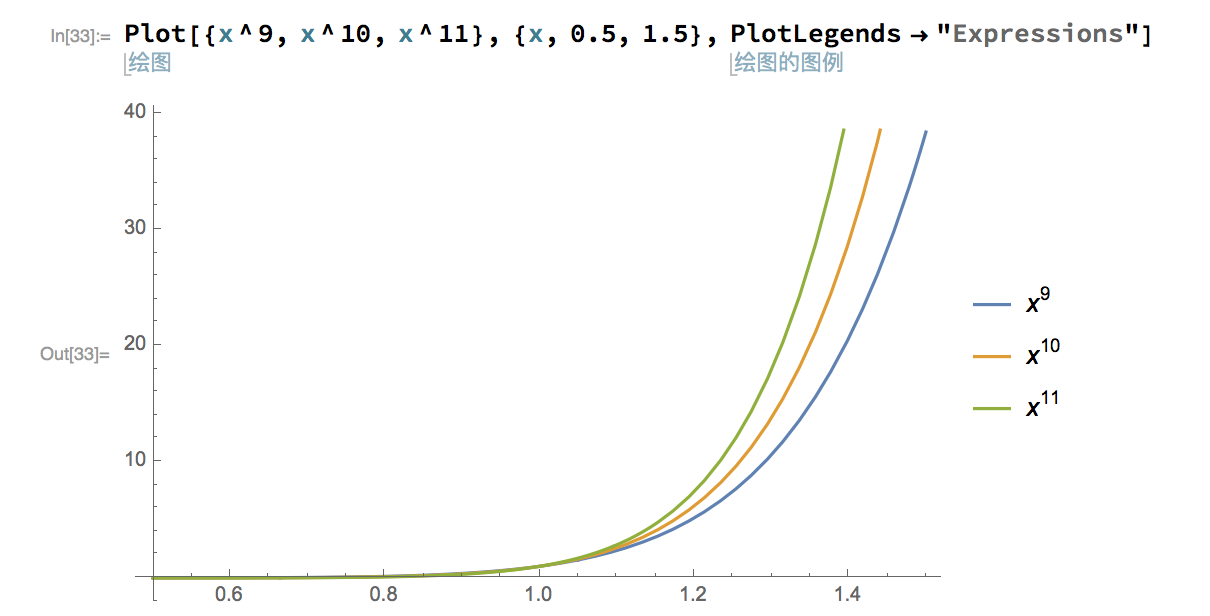
\includegraphics[width=12cm]{./Figures/20170917-monomial-mcl}
  \label{fig:pj-spectral-monomials}
%
%  \small{Source: PBOC.}
\end{figure}



单项式基的上述缺点,使得我们寻求利用正交多项式构建基方程。内积形式的正交多项式的值相对于$x$的变化往往较为平缓,并且在加入更高次多项式元素后,系统会出现足够大的变化,有助于更精确近似原系统中的方程$d(\cdot)$。

\subsection{三角序列}
\label{sec:pj-base-spectral-trigonometric}
光谱法全局基的另一选项是三角序列(trigonometric series)\index{basis!trigonometric series \dotfill 三角序列(基)},如
\begin{equation*}
  \frac{1}{\sqrt{2 \pi}},
  \frac{\cos x}{\sqrt{2 \pi}},
  \frac{\sin x}{\sqrt{2 \pi}},
  \ldots,
  \frac{\cos k x}{\sqrt{2 \pi}},
  \frac{\sin k x}{\sqrt{2 \pi}},
  \ldots
\end{equation*}

三角序列适合用于分析有周期性特征的方程,因而在自然科学和工程学中得到广泛应用。遗憾的是除了时间序列分析等领域之外,经济学研究的问题较少涉及到周期性。此外,目前将周期性方程近似为非周期性方程的方法尚未成熟。因此我们不做深入探讨。

\subsection{雅各比多项式}
\label{sec:pj-base-spectral-jacobi-poly}
雅各比多项式\index{basis!Jacobi polynomial \dotfill 雅各比多项式(基)}(第\ref{sec:poly-jacobi-polynomial}节)也适合作为光谱法全局基的选项之一。

雅各比多项式一族中,还包括盖根鲍尔多项式(Gegenbauer), 勒让德(Legendre),切比雪夫多项式(Chebyshev),他们可以相互转换。\cite[Table 1]{Boyd:2013kj}比较了几种多项式在处理不同优化指标时的性能排序,从而提供了重要参考:在绝大多数情况下,对于求解DSGE模型的工作来说,最适于采用切比雪夫多项式构建基方程。

\subsection{切比雪夫多项式}
\label{sec:pj-base-spectral-chebyshev-poly}
切比雪夫多项式\index{basis!Chebyshev polynomial \dotfill 切比雪夫多项式(基)}(第\ref{sec:poly-chebyshev-polynomial}节)作为光谱法全局基的选项之一,具有许多优点:
\begin{enumerate}
  \item 便于在各种表述形式之间互相转换,如罗德里格斯公式、三项递推关系、母方程
  、二阶导数线性方程等。
  \item 可以通过余弦换算,迅速计算系数变化后的值。
  \item 切比雪夫插值(interpolation)换算的结果,比其他几种多项式插值的结果更为稳健。
  \item 切比雪夫多项式是平滑的,并且有界(闭区间$[-1,1]$)。
  \item 切比雪夫差值的误差,可以由一系列定理得到较好的限制。
\end{enumerate}

第一类切比雪夫多项式$T_n(x)$满足关系$T_n(0)=1, T_n(1)=x, T_{n+1}(x) = 2x T_n(x) - T_{n-1}(x)$,因此我们可得到一组多项式序列$1, x, 2x^2-1, 4x^3 - 3x, 8x^4 - 8x^2 + 1, \ldots$,随着$n=0,1,2,\ldots,7$,我们绘制出了$T_n(x)$的曲线,见\ref{fig:pj-spectral-chebyshev}。不难看出,$n=0$时是条平行线,$n=1$时是$45$度斜线,$n=2$时是一条抛物线,随着$n$逐渐增加,切比雪夫多项式的曲线形状呈波浪状。
\begin{figure}[htbp]
   \caption{切比雪夫多项式$T_n(x)$}
  \centering
  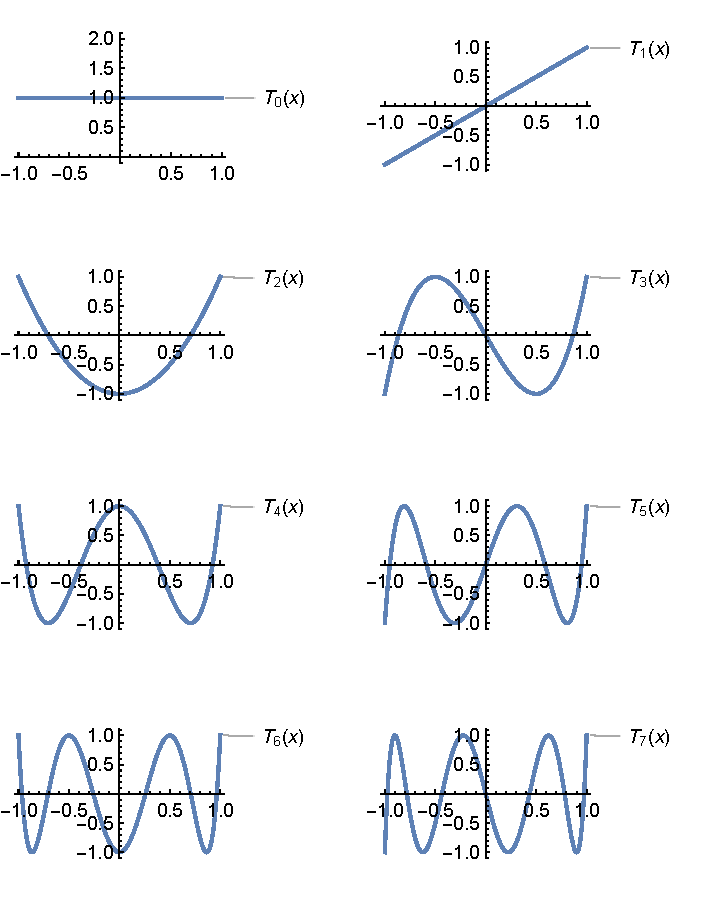
\includegraphics[width=15cm]{./Figures/20170917-chebyshev-poly}
  \label{fig:pj-spectral-chebyshev}
%
%  \small{Source: PBOC.}
\end{figure}

图\ref{fig:pj-spectral-chebyshev}在Mathematica中输入如下命令生成:
\begin{verbatim}
  t0 = Plot[{ChebyshevT[0, x]}, {x, -1, 1}, PlotLabels -> "Expressions"];
  t1 = Plot[{ChebyshevT[1, x]}, {x, -1, 1}, PlotLabels -> "Expressions"];
  t2 = Plot[{ChebyshevT[2, x]}, {x, -1, 1}, PlotLabels -> "Expressions"];
  t3 = Plot[{ChebyshevT[3, x]}, {x, -1, 1}, PlotLabels -> "Expressions"];
  t4 = Plot[{ChebyshevT[4, x]}, {x, -1, 1}, PlotLabels -> "Expressions"];
  t5 = Plot[{ChebyshevT[5, x]}, {x, -1, 1}, PlotLabels -> "Expressions"];
  t6 = Plot[{ChebyshevT[6, x]}, {x, -1, 1}, PlotLabels -> "Expressions"];
  t7 = Plot[{ChebyshevT[7, x]}, {x, -1, 1}, PlotLabels -> "Expressions"];
  GraphicsGrid[{{t0, t1}, {t2, t3}, {t4, t5}, {t6, t7}}]
\end{verbatim}


第$n$次切比雪夫多项式$T_n(x)$有$n$个根,对应
\begin{equation}
  \label{eq:pj-spectral-cheby-roots-n}
  x_k = \cos \left( \frac{2k - 1}{2n} \pi \right), \quad k = 1, 2, \ldots, n, -1 \le x_k \le 1,
\end{equation}
如图\ref{fig:pj-spectral-cheby-roots-n}所示,所有根都在闭区间$[-1,1]$之间。
\begin{figure}[htbp]
   \caption[切比雪夫多项式的根]{切比雪夫多项式$T_n(x)$的根$x_k, n=100, k=1,2,\ldots,n$}
  \centering
  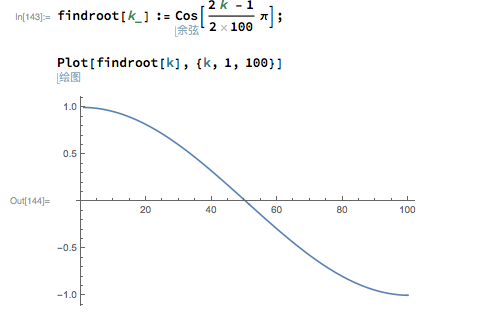
\includegraphics[width=8cm]{./Figures/20170917-cheb-roots-n-range}
  \label{fig:pj-spectral-cheby-roots-n}

  \small{说明:计算等式依据\eqref{eq:pj-spectral-cheby-roots-n}。}
\end{figure}

大多数DSGE模型的状态变量域$x \in [a,b]$,$a,b \neq \pm 1$,在实际研究中我们常采用如下线性关系转换,将它转换为$[-1,1]$区间内的值,以符合切比雪夫多项式的要求:
\begin{equation}
  \label{eq:pj-state-transformation-chebysev-interval}
  2 \frac{x-a}{b-a} -1,
\end{equation}
详见第\ref{sec:pj-spectral-cheby-variable-change}节。
例如$(a=-7,b=5)$的某状态变量线性转换,如图\eqref{fig:pj-state-transformation-chebysev-interval}所示。
\begin{figure}[htbp]
   \caption[切比雪夫多项式的根]{切比雪夫多项式$T_n(x)$的根$x_k, n=100, k=1,2,\ldots,n$}
  \centering
  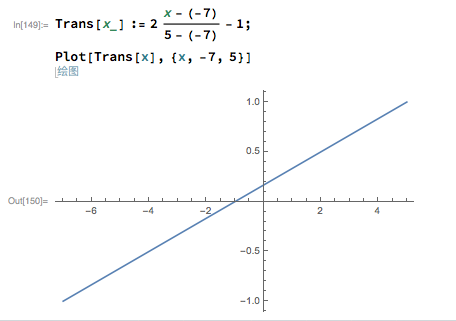
\includegraphics[width=8cm]{./Figures/20170917-linear-trans-state-chebyshev}
  \label{fig:pj-state-transformation-chebysev-interval}

  \small{说明:计算等式依据\eqref{eq:pj-state-transformation-chebysev-interval}。}
\end{figure}

使用切比雪夫多项式作为映射基,有两个定理值得关注:
\begin{enumerate}
  \item 切比雪夫插值定理(Chebyshev interpolation theorem)\index{interpolation!Chebyshev \dotfill 切比雪夫插值},见附录\ref{sec:poly-chebyshev-interpolation}:如果近似方程恰好是第$n_1$次切比雪夫多项式的根,那么随着$n_1 \rightarrow \infty$,近似误差逐渐减少到足够小的程度。根据切比雪夫插值定理,可以使用切比雪夫多项式的根作为正交配点(orthogonal collocation) \index{collocation! \dotfill 配点}\index{collocation!orthogonal \dotfill 正交配点},见\ref{sec:pj-fem}节FEM方法介绍。
  \item 切比雪夫截断定理(Chebyshev truncation theorem)\index{truncation!Chebyshev \dotfill 切比雪夫截断},见附录\ref{theorem:poly-cheby-truncation-theorem}。进而在特定情况下,切比雪夫向未知原方程做几何收敛(geometric convergence),可以表示为
  \begin{equation*}
    d(x) - d^j(x | \theta) \sim \bm{O}(\theta_j),
  \end{equation*}
  即是说,当切比雪夫近似停止于第$j$次多项式时,对应的截断误差与$j$次切比雪夫多项式系数$\theta_j$是同次的。

  根据该定理,我们可以设计一种数值检测机制:如截断误差大于某一阈值,则意味着$j$次切比雪夫近似$T_j(x)$的精度不够,需要再增加一次近似至$T_{j+1}(x)$。我们将在下文进一步讨论该问题\todo{reference}。
\end{enumerate}

\subsubsection{变量的变换}
\label{sec:pj-spectral-cheby-variable-change}

如前所述,\ref{eq:pj-state-transformation-chebysev-interval}提供了一种可将$x \in [a,b], a < -1, b > 1$转化为$[-1,1]$区间中变量的方法,以便进行切比雪夫多项式近似。在扰动法中我们也讨论了变量的变换,见\ref{sec:perturbation-change-variables}节。二者尽管技术细节有所不同,但核心思路是相同的:都是为了尽可能提高近似的精确度。本节以随机NCGT模型为例,介绍为何通过变量变化有助于提高映射法的近似精度。

原目标为寻找经济系统方程组
\begin{align*}
  &c_t = d^1(k_t,z_t), \\
  &k_{t+1} = d^2(k_t,z_t)
\end{align*}
的近似解。我们可以通过变量变换,改为寻求方程组
\begin{align*}
  &\log c_t = d^1(\log k_t, z_t),\\
  &\log k_{t+1} = d^2 (\log k_{t}, z_t)
\end{align*}
的近似解,用映射法表示为
\begin{align*}
  &\log c_t = d^{1,j}(\log k_t, z_t|\theta^1) = \sum_{i=0}^{j} \theta^1_i \psi_i (\log k_t, z_t),\\
  &\log k_{t+1} = d^{2,j} (\log k_{t}, z_t | \theta^2 ) = \sum_{i=0}^{j} \theta_i^2 \psi_i (\log k_t, z_t).
\end{align*}

\subsubsection{伯依德原则}
前文简要介绍了利用切比雪夫多项式从事经济学研究所具有的理论优势。但近些年来的经验研究,尤其是基于DSGE模型的经济学研究,越来越多地使用基于切比雪夫多项式的映射法,切比雪夫多项式作为基方程的备选方案,其巨大优势得到了越来越广泛的认可\citep{Aruoba:2006cz,Caldara:2012fr}。

\cite[p.10]{Boyd:2001wt}用一种近似于开玩笑的方式,总结了这几十年来的研究经验,将之命名为``道德准则一号'':
\begin{enumerate}
  \item 当不确定用什么基时,就用切比雪夫多项式。除非模型呈现出较强的周期性,这时可以考虑用傅里叶序列。
  \item 除非你确定其他某种基方程更好,不然就用切比雪夫多项式。
  \item 除非你非常非常确定其他某种基方程更好,不然就用切比雪夫多项式。
\end{enumerate}

\section{局部基的选取(1)}
\label{sec:pj-method-local}

第\ref{sec:pj-spectral-method-global}节所介绍的几种方案,全部都是单维度基方程,相对简单,易于我们理解用映射法求解DSGE模型的基本思路。然而现实世界中大多数经济问题都是多维度的,几乎全部DSGE模型都研究一个以上的状态变量。这就需要我们探讨多维基的选择方案。

如何选取多维基成为映射法的关键问题。然而映射法受到维度灾难(curse of dimensionality)\index{curse of dimensionality \dotfill 维度灾难}的强烈冲击\citep{Bellman:1957tx}。随着解释变量数量的增加——如中等规模DSGE模型可能要处理超过20组解释变量——应用映射法求解模型变得异常困难,这要求我们用更高的技巧去选取多维基方程。

\subsection{离散状态变量}
\label{sec:pj-multidimen-discrete-state-variables}
前文一系列分析均暗含假定,状态变量是连续的。然而在很多DSGE模型中,至少一部分变量是离散的:
\begin{itemize}
  \item 状态变量本身是离散的,如
  \begin{itemize}
    \item 财政政策,政府可能处于主权债务违约或未违约状态\citep{Bocola:2016ij},
    \item 货币政策,可能是积极的或者消极的\citep{Leeper:1991kq},
  \end{itemize}
  \item 出于计算求解的考虑,益于将连续状态变量做离散化处理,如
  \begin{itemize}
    \item 外生随机过程(技术冲击、偏好冲击等)的离散化。
  \end{itemize}
\end{itemize}

研究发现,有限马尔科夫链(finite Markov chain)\index{Markov chain!finite \dotfill 有限马尔科夫链}能够产生与连续过程相同的样本矩;经验分析表明,在大多数情况下,含有5-7个状态的马尔科夫链足够模拟一般情况下的随机过程信息,供经济学定量分析使用\citep{Tauchen:1986gi, Kopecky:2010du}。因此状态变量的离散化问题可以理解为,针对某一个连续变量,我们寻找另一个(离散的)决策方程来描述它\footnote{我们不对马尔科夫链做过多介绍(来不及把笔记敲进硬盘了)。讲义可参考帝国理工大学Emma J McCoy M3S4/M4S4 - Applied Probability的讲义第六章:Markov Chains, \url{http://101.96.10.63/wwwf.imperial.ac.uk/~ejm/M3S4/NOTES3.pdf}。教材可参考\cite{Privault:2013vc}。}。

仍然以含有随机NCGT模型为例,假定外生技术冲击$z_t$是一个一阶自回归过程$AR(1)$
\begin{equation*}
  z_t = \rho z_{t-1} + \varepsilon_t,
\end{equation*}
其中$\varepsilon_t \sim N(0,\sigma^2_z)$是一个平稳分布(stationary distribution)\index{distribution!stationary \dotfill 平稳分布}。

可以表示为含有$n$个点的马尔科夫过程$z_t \in \{ z_1, z_2, \ldots z_n \}$,对应转移矩阵$P_{z,z'}$ (transition matrix)\index{transition matrix \dotfill 转移矩阵}
\begin{equation}
  \label{pj-discrete-transition-matrix-def}
  P_{z,z'}=\begin{pmatrix}
  p_{11}& \ldots &p_{1n} \\
  p_{21}& \ldots &p_{2n} \\
  \vdots& \ddots & \vdots \\
  p_{n1} & \ldots & p_{nn}
  \end{pmatrix},
\end{equation}
其中转移概率(transition probability)\index{transition probability \dotfill 转移概率} $p_{i,j}$ 表示当前期处于位置$i$马尔科夫链下一时期转移到位置$j$的概率。

将AR(1)过程$z_t$离散化的常见算法,见附录第\ref{sec:pj-local-discretization}节。

(注意,建议阅读这个附录,以便弄明白是怎么回事,还有附带的matlab代码。)

将技术冲击离散化后,我们的研究目标就变为,寻找$2 \times n$个决策方程:
\begin{equation*}
  \begin{split}
    &c \left( k, z_m \right) = d^{c,m,j} \left( k | \theta^{m,c} \right) = \sum_{i=0}^{j} \theta_{i}^{m,c} \psi_i(k), \\
    &k \left( k, z_m \right) = d^{k,m,j} \left( k | \theta^{m,k} \right) = \sum_{i=0}^{j} \theta_{i}^{m,k} \psi_i(k),
  \end{split}
\end{equation*}
其中$m=1,2,\ldots,n$。举例来说,我们首先寻找当今天的技术水平是$z_1$时资本和消费的决策方程,进而寻找当今天的技术水平是$z_2$时资本和消费的决策方程,随后$z_3, \ldots, z_m, \ldots, z_n$。为了让数值运算不至于太过复杂,我们常将$n$控制在一个比较小的值上,比如5到7之间。

在求得两个决策方程后,代回到原系统的欧拉方程
\begin{equation}
  \label{eq:pj-local-euler-eq}
  u'(c_t) = \beta E_t \left[ u'\left( c_{t+1} \right) \left( \alpha \exp(z_{t+1}) k_{t+1}^{\alpha - 1} + 1 - \delta \right) \right]
\end{equation}
中,我们有
\begin{equation}
  \label{eq:pj-local-euler-eq-discrete}
  \begin{split}
    u'\left( d^{c,m,j} \left( k | \theta^{m,c} \right)\right) = \beta \sum_{l=0}^{n} p_{ml} &\left[
    u'\left(
    d^{c,l,j}
    \left( d^{k,m,j} \left( k | \theta^{m,k} \right) | \theta^{l,c} \right)
     \right) \right. \\
     & \left. \left(
     \alpha \exp(z_{t+1})
     \left(
     d^{k,m,j} \left( k | \theta^{m,k} \right)
    \right)^{\alpha-1}
     + 1 - \delta
     \right)
    \right]
  \end{split}
\end{equation}

\eqref{eq:pj-local-euler-eq-discrete}中有两点值得注意
\begin{enumerate}
  \item 近似算法中$2 \times n$个决策方程都是当期的,不过上式中$t+1$的决策方程,依然考虑到$t+1$期可能出现的技术水平变化。
  \item  由于我们将随机过程进行离散化近似,对应地,积分形式的RHS被简化为离散求和形式,乘以转移矩阵\eqref{pj-discrete-transition-matrix-def}中的相应元素\footnote{也有一些研究直接从积分形式入手,探讨一系列求积法,可参考\cite{Judd:1998uy,Judd:2011iw}。}。
\end{enumerate}

因此,在存在多维度问题的DSGE模型中,常常可以对其中至少一部分状态变量如技术冲击做离散化处理,其优点在于简单直观,操作过程透明,并且不是特别耗费计算资源。以及在一定意义上,求解DSGE模型往往依赖于混合策略:对一部分连续状态变量做离散化处理,对剩余的连续变量采用其他近似策略,如张量、完全多项式等,见下文。


\subsection{张量与完全多项式}
\label{sec:pj-multidimen-tensor}
张量(tensors)\index{tensor \dotfill 张量}将一组单维的基方程,用克罗内克乘积\index{Kronecker product \dotfill 克罗内克乘积}的组合在一起,构成多维基方程。例如一个经济系统中有两个状态变量,实物资本$k_t$和人力资本$h_t$,每个状态变量分别对应3个切比雪夫多项式:
\begin{equation*}
  \begin{split}
    &\psi_{0}^k(k_t),\psi_{1}^k(k_t),\psi_{2}^k(k_t),\\
    &\psi_{0}^h(h_t),\psi_{1}^h(h_t),\psi_{2}^h(h_t).
  \end{split}
\end{equation*}

则我们可以构建一个张量作为基方程
\begin{equation*}
  \begin{split}
    &\psi_{0}^{k}(k_t) \psi_{0}^{h}(h_t),
    \psi_{0}^{k}(k_t) \psi_{1}^{h}(h_t),
    \psi_{0}^{k}(k_t) \psi_{2}^{h}(h_t), \\
    &\psi_{1}^{k}(k_t) \psi_{0}^{h}(h_t),
    \psi_{1}^{k}(k_t) \psi_{1}^{h}(h_t),
    \psi_{1}^{k}(k_t) \psi_{2}^{h}(h_t), \\
    &\psi_{2}^{k}(k_t) \psi_{0}^{h}(h_t),
    \psi_{2}^{k}(k_t) \psi_{1}^{h}(h_t),
    \psi_{2}^{k}(k_t) \psi_{2}^{h}(h_t).
  \end{split}
\end{equation*}

进而,对于一个有$n$个状态变量的方程系统$d:[-1,1]^n \rightarrow \mathbb{R}$,我们试图用$j$次切比雪夫多项式予以近似,则可用如下张量形式表现
\begin{equation*}
  d^j(\cdot | \theta) = \sum_{i_1 = 0}^{j} \sum_{i_2 = 0}^{j} \ldots \sum_{i_n = 0}^{j} \theta_{i_1, i_2, \ldots, i_n} \, \psi_{i_1}^{1}(\cdot) * \ldots  \psi_{i_n}^{n}(\cdot),
\end{equation*}
其中$\psi_{i_\kappa}^{\kappa}$是第$\kappa$个状态变量的$i_{\kappa}$次切比雪夫多项式,$\kappa = 1,2,\ldots,n$;系数向量$\theta$为$\left\{ \theta_{i_1}, \theta_{i_2}, \ldots, \theta_{i_n} \right\}$。

采用张量基方程有如下优点,
\begin{enumerate}
  \item 易于构建
  \item 传递性:如果组成张量的单维基方程是正交的,那么由单维基乘积组成的张量基方程也是正交的。
\end{enumerate}
最显著的不足在于维数灾难\index{curse of dimensionality \dotfill 维数灾难}:待求解系数$\theta_{i_1, \ldots i_{n}}$的个数随着$j$和$n$的增加而指数增加,呈$(j+1)^n$形。上例中$j=2,n=2$对应需要近似计算$9$个系数;图\ref{fig:pj-local-tensor-simu}。
\begin{equation*}
(j+1)^n =
\begin{cases}
    256 & (j,n)=(3,4)\\
    3125 & (j,n)=(4,5)\\
    46656 & (j,n)=(5,6)\\
    \ldots
\end{cases}
\end{equation*}
\begin{figure}[htbp]
   \caption[张量模拟]{张量代求解系数的数量$(j=1)^n$}
  \centering
  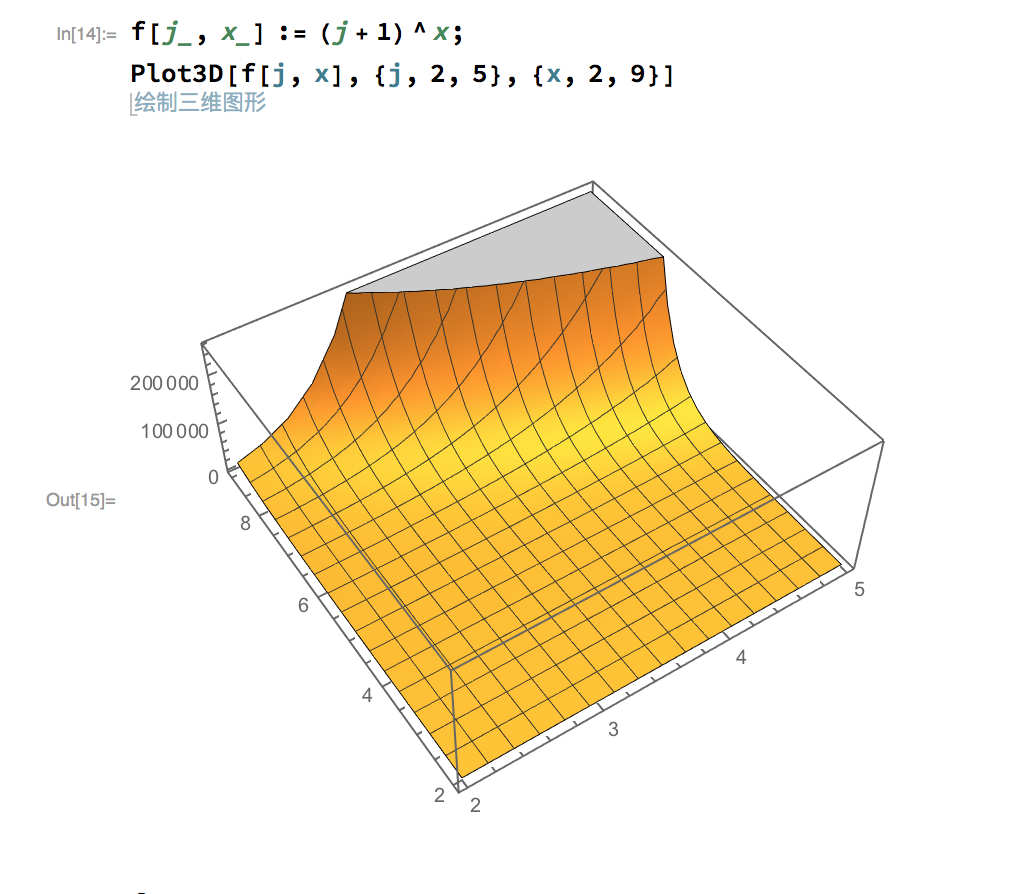
\includegraphics[width=8cm]{./Figures/20170920-tensor-coefficient}
  \label{fig:pj-local-tensor-simu}
%
%  \small{Source: PBOC.}
\end{figure}

在实际研究中,当模型里有$n>3$个连续状态变量和1个哪怕是中等规模的$j$时,张量基的方法便不易展开了。一个方法是去掉张量集合中的部分元素,以减轻计算负担。\cite{Gaspar:1997we}建议使用完全多项式(complete polynomials)\index{polynomial!complete \dotfill 完全多项式}:
\begin{equation}
\begin{split}
    \mathcal{P}^n_{\kappa} \equiv & \left\{ \psi_{i_1}^1 * \ldots * \psi_{i_n}^n \right\}, \left| \bm{i} \right| \le \kappa ,\\
    & \left| \bm{i} \right| = \sum_{l=1}^n i_l, \quad 0 \le i_1,\ldots,i_n,
\end{split}
\end{equation}
即是说,首先预设一个正整数值$\kappa$,进而在张量中,只选取各个基方程的级数之和小于$\kappa$所对应的那部分元素。这是基于下述认识:对于描述原方程系统$d$的目标而言,绝大多数信息都已经在完全多项式$\mathcal{P}^n_{\kappa}$中体现出来了;余下的部分$ \psi_{i_1}^1 * \ldots * \psi_{i_n}^n, \left| \bm{i} \right| > \kappa $ 只能给基方程产生有限的信息,却是以大量额外计算时间为代价的。

举例来说,对于$j=4,n=3$的张量系统,有$(4+1)^3=125$个元素。我们设$\kappa = 6$,提取$\left| \bm{i} \right| \le 6$的部分构建完全多项式$\mathcal{P}_6^3$,则只需要近似计算其中的87个系数了。

不幸的是,这仍然太多。在下文\todo{reference}中我们进一步介绍斯莫尔亚克稀疏网格算法。

\section{局部基的选取(2):有限元法}
\label{sec:pj-fem}

作为局部基方法的一种,有限元法(finite elements method, FEM)\index{finite elements method \dotfill 有限元法} 由\cite{McGrattan:1996gu}最先在经济学研究中倡导并予以实践\footnote{有限元法的数理知识,可见教材\cite{Hughes:2000ve, Brenner:2008hf}。可参考Joseph E. Flaherty的讲义 CSCI, MATH 6860: Finite Element Analysis \url{http://www.cs.rpi.edu/~flaherje/FEM/index4.html}。}。

有限元法常应用在一些关键任务的工业领域,如航空航天,核电厂施工等,这是由它的突出优势所决定的:可以很方便描述某些局部域内的行为,以及达到相当高的精确度。相应地,有限元法的主要不足在于难以编程,计算求解速度慢。

利用有限元法展开分析,常见的步骤如下。第一步是确定状态变量的值域$\Omega$。值域的选取方面,一些规则是天然的(如$k_t > 0$),另一些则不是($k_t < \bar{k}$),后者我们需要额外注意:如,可以将$\bar{k}$设的足够高,以至于在模型仿真过程中所有$k_t$都在上限$\bar{k}$的下方。随着仿真过程的实际展开,$\bar{k}$的值也可能做微调。

第二步是将$\Omega$分成若彼此不重叠的有限个元。各个元相接的部分称为节点(nodes)\index{node \dotfill 节点}。分元的原则总体上来讲灵活性很高,可以
\begin{itemize}
  \item 均等划分,直观简便
  \item 根据变量处于某种状态的频率,划分为一系列小块(频率高)和大块(频率低)。对``频率''的设定又分为两种情况
  \begin{itemize}
    \item 来自理论模型系统的特征
    \item 利用迭代法,对所划分元的事后验证\todo{见下文,补reference。}
  \end{itemize}
  \item 在$\Omega$中,将$d(\cdot)$变化幅度较大的部分划分为小元,相对变化幅度不大的部分划分为大元,从而在每一个元内部,原本是非线性的$d(\cdot)$接近线性。
\end{itemize}

在工程实践中,得益于灵活的分元,有限元法可以更好处理kinks或者一些特殊限制条件\footnote{kinks通常是指,分元后,两个元的衔接处 (interface) 出现偏移(弱kinks)甚至断裂(强kinks)的情况,见图\ref{fig:pj-kinks}。}。面对这些kinks、或限制条件,一方面光谱法的操作难度较大,另一方面由于不满足可微、连续等条件,扰动法很难展开。
\begin{figure}[htbp]
   \caption[kinks]{弱kinks和强kinks的示例图}
  \centering
  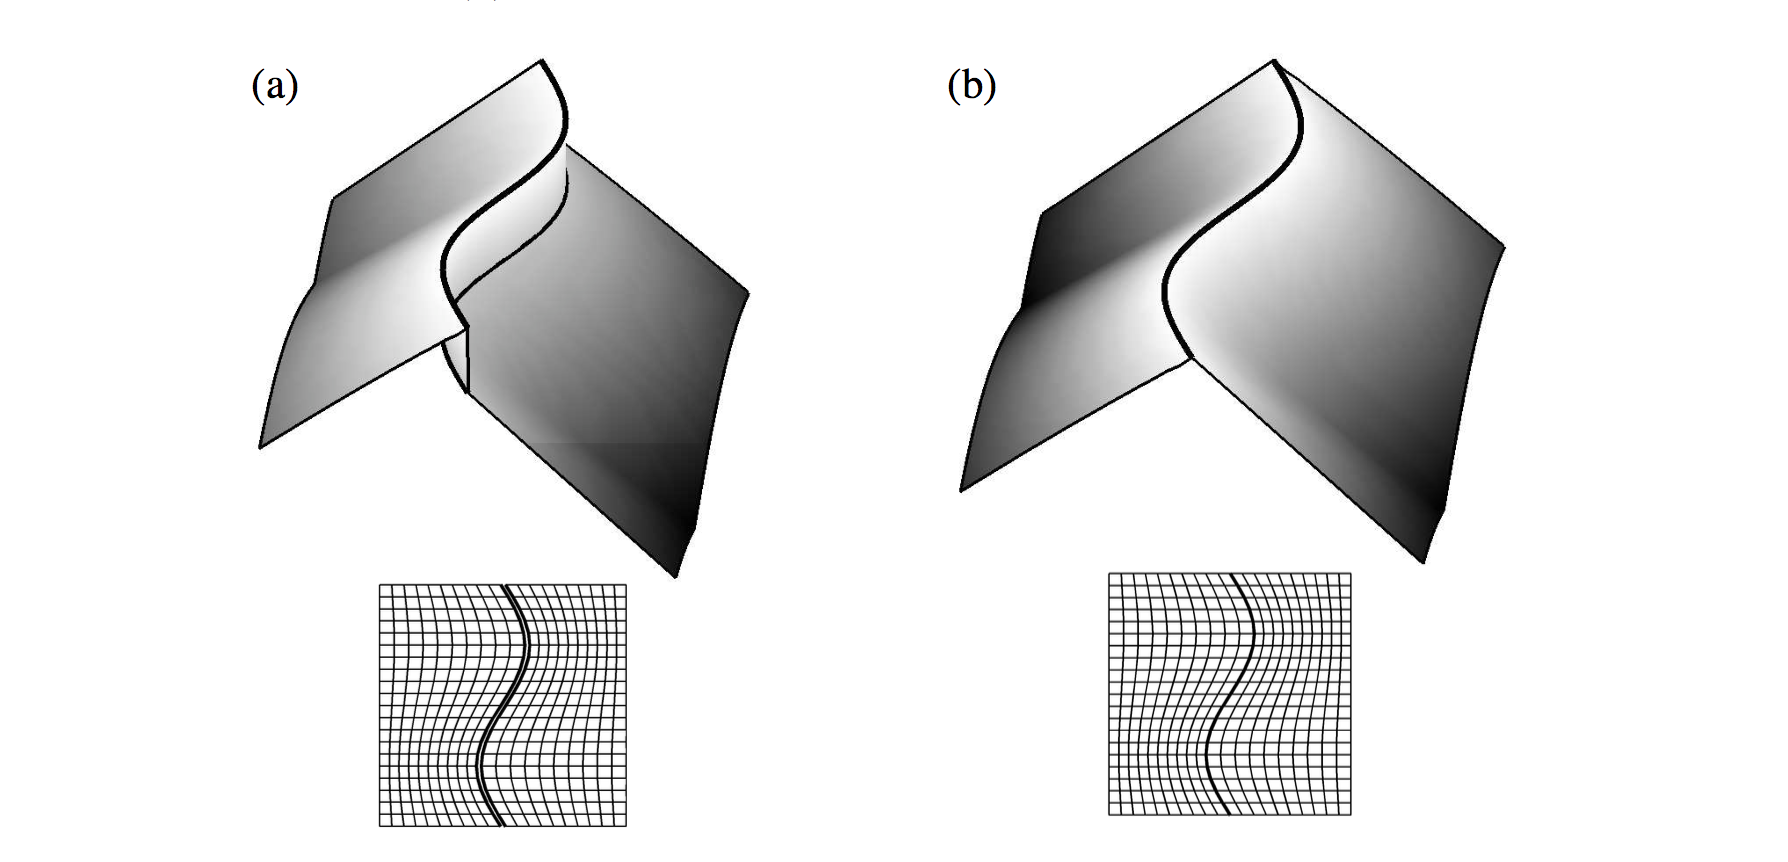
\includegraphics[width=10cm]{./Figures/20170921-kinks-fem}
  \label{fig:pj-kinks}

  \small{图片来源:\cite[Figure 2]{Fries:2010hj}。}
\end{figure}

将$\Omega$域分为有限个元素的的最优方法(网格生成 grid generation \index{grid \dotfill 网格}),已有大量工程学、数学方面的讨论,如\cite{Thompson:1985ug}。在内生NCGT模型中应用网格优化法生成有限个不均等的元以优化计算时间,可见\cite{FernandezVillaverde:2004fg}。

第三步,在每一个元中选择对应的基,用于构建政策方程。如果前述步骤中元素的划分已经有效,则这一步中的基只设定线性形式即可。例如,$\Omega$中诸元的节点表示为$\{k_0, k_1, \ldots k_j\}$,则可以定义基方程$\psi_{i}(k)$为三角函数形式,$i = 1,2,\ldots,j-1$:
\begin{subequations}
\label{eq:pj-fem-base-tent}
\begin{align}
  \label{eq:pj-fem-base-tent-a}
  &\psi_0(k) =
  \begin{cases}
  \frac{k_0 - k}{k_1-k} , \text{如果} k \in [k_0,k_1], \\
  0,
  \end{cases} \\
  \label{eq:pj-fem-base-tent-b}
  &\psi_i(k) =
  \begin{cases}
    \frac{k - k_{i-1}}{k_i - k_{i-1}}, \text{如果} k \in [k_{i-1},k_{i}],\\
    \frac{k_{i+1} - k}{k_{i+1} - k_i}, \text{如果} k \in [k_{i},k_{i+1}], \\
    0,
  \end{cases}\\
  \label{eq:pj-fem-base-tent-c}
  &\psi_j(k) =
  \begin{cases}
  \frac{k - k_{j-1}}{k_{j}-k_{j-1}}, \text{如果} k \in [k_{j-1},k_{j}],\\
  0.
  \end{cases}
\end{align}
\end{subequations}

之所以说\eqref{eq:pj-fem-base-tent}的基方程是三角形式,举例说明,见图\ref{fig:pj-fem-tent}。
\begin{figure}[htbp]
   \caption{三角方程形式}
  \centering
  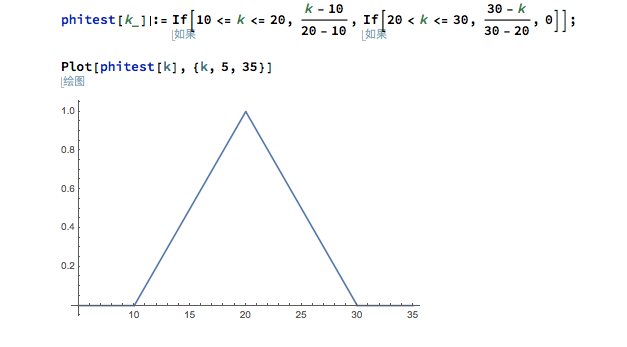
\includegraphics[width=10cm]{./Figures/20170921-tent-function}
  \label{fig:pj-fem-tent}
%
%  \small{Source: PBOC.}
\end{figure}

第四步,与其他映射法类似,生成决策方程系统作为原方程系统的近似,在有限元分析中我们常称之为分段线性近似(piecewise linear approximation)。
\begin{equation*}
  d^{n,j}\left( \cdot | \theta^n \right) = \sum_{i=0}^{j} \theta^n_i \psi_{i} \left( \cdot \right),
\end{equation*}
将近似系统代回$\mathcal{H}$。其中,$\theta$和$\psi$由切比雪夫多项式的相关算法求得:以本例中的有限元节点$k_i$和$k_{i+1}$为例,分别对应基方程
\begin{equation*}
  \begin{split}
    \psi_{i}(k) = \frac{k_{i+1} - k}{k_{i+1} - k_{i}}, \\
    \psi_{i+1}(k) = \frac{k - k_{i}}{k_{i+1} - k_i},
  \end{split}
\end{equation*}
那么由节点$k_i$和$k_{i+1}$划出的元中,值$d^{n,j}\left( \cdot | \theta^n \right)$由一个近似方程$\hat{d}$表示
\begin{equation*}
\begin{split}
    \hat{d} \left( k | k_{i}, k_{i+1}, \theta^n_i, \theta^n_{i+1} \right) &= \theta_i^n \psi_i(k) + \theta_{i+1}^n \psi_{i+1}(k) =\theta_i^n \frac{k_{i+1} - k}{k_{i+1} - k_{i}} + \theta_{i+1}^n \frac{k - k_{i}}{k_{i+1} - k_i} \\
    &= \frac{
    \left( \theta_{i+1}^n - \theta_{i}^n \right) k + \theta_{i}^n k_{i+1} - \theta_{i+1}^n k_{i}
    }{k_{i+1} - k_i},
\end{split}
\end{equation*}
不难看出,近似方程$\hat{d}$是线性的,斜率的符号由$\theta_{i+1}^n - \theta_{i}^n$来决定。

另一方面采用类似的方法,以有限元节点$k_{i-1}$和$k_{i}$划出的元中,我们可以得到另一个线性近似方程$\hat{d}$
\begin{equation*}
  \hat{d} \left( k | k_{i-1}, k_{i}, \theta^n_{i-1}, \theta^n_{i} \right)=
  \frac{
  \left( \theta_{i}^n - \theta_{i-1}^n \right) k + \theta_{i-1}^n k_{i} - \theta_{i}^n k_{i-1}
  }{k_{i} - k_{i-1}}。
\end{equation*}

两个元在$k_i$处相交,此时我们有
\begin{equation*}
  \begin{cases}
    \hat{d} \left( k_{i} | k_{i}, k_{i+1}, \theta^n_i, \theta^n_{i+1} \right)  = \theta^n_i, \\
    \hat{d} \left( k_i | k_{i-1}, k_{i}, \theta^n_{i-1}, \theta^n_{i} \right)= \theta^n_i,
  \end{cases}
\end{equation*}
即两个方程等于一个相同的值$\theta^n_i$,这确保了作为各个$\hat{d}$的加总的$d$方程是连续的。

上述介绍也说明为何有限元法提供的分段线性近似\index{piecewise linear approximation \dotfill 分段线性近似}是个较为理想的近似策略。假定我们设对应的度量方程$\rho(\cdot)$的形式为\footnote{度量方程的选取方案有数种,这里只举其中之一;更多讨论见下节。}\todo{reference},使得在划分元所依据的每个节点$k_i$上,都有残差方程$R(\cdot) = 0$。对于三角函数形式的分段基方程$\psi_i(\cdot)$而言,这意味着当状态变量处在$k_i$节点上时,对系数$\theta^n_i$的取值应当使得近似方程系统与原方程系统相等:
\begin{equation*}
  \hat{d}^{n,j}(\cdot | \theta^n) = d^n(\cdot).
\end{equation*}

需要指出的是,有限元分析中的分段线性近似法也表明,系数$\theta^n_i$的选取,与状态变量处于节点$k_i$之外其他位置时$d^n(\cdot)$的值无关。从这个意义上来讲,利用有限元法求解大型非线性方程系统所得到的近似系统,都是稀疏的(sparse)。这成为一个可为现代非线性求解方法所利用的特征。

第五步,(如有需要)对结果的改进。如果第一轮有限元分析近似解的精度不达标,我们可以根据需要对近似解做反复改进,进行第二轮、第三轮甚至更多有限元分析,在计算时间和内存允许的范围内,尽可能提高近似解的精度。事实上这是有限元法研究的又一突出优势。在现有研究文献中,改进常常分为三大类型。
\begin{enumerate}
  \item h——改进(h-refinement)\index{h-refinement finite elements\dotfill h——改进(有限元分析)},在全部域$\Omega$内,将第一轮所分元(如$A,B,C, \ldots$)再均等分为更小的元(如$A1,A2,A3, \ldots$),对这些细分元再反复迭代使用有限元法,改善近似解,直至精度达标。
  \item r——改进(r-refinement)\index{r-refinement finite elements \dotfill r——改进(有限元分析)},第二、第三甚至更多轮有限元分解的重点针对存在着明显非线性特征的局部。
  \item p——改进(p-refinement)\index{p-refinement finite elements \dotfill p——改进(有限元分析)},不对现有元再作细分,而是在元内部通过加入更多个基方程(如更多的切比雪夫多项式)来提高近似的阶数(order);如果元内现有阶数已足够高,则应用有限元法和光谱法组合的混合策略,常称为光谱元法(spectral elements)\index{spectral elements \dotfill 光谱元}。在自然科学和工程学领域,光谱元法已得到了广泛应用\citep{Solin:2003up}。
\end{enumerate}

有时,h——和p——改进被混合在一起使用,称hp——有限元法(hp-adaptive finite elements)\index{hp-adaptive finite elements \dotfill hp——有限元法},可以使近似解以指数速度向真实解收敛\citep{Ciarlet:2002tm}。尽管它的编程难度更高,计算时间更长,但hp——有限元法可能是目前已知最强大的DSGE求解工具了,有助于求解甚至是最复杂的DSGE模型。关于这种方法的详细介绍,可参考\cite{Babuska:1994jz,Demkowicz:2006ww,Demkowicz:2007ur}。

\section{目标方程的选取}
\label{eq:pj-metric}
如前所述,映射法研究中也需要选取度量方程$\rho$作为目标方程。在未对$\mathcal{H}$作过多限定的前提下,可视$R(\cdot | \theta)$为最简单的单维情况\footnote{随着$\mathcal{H}$的限定条件变多,$R(\cdot \theta) = \mathcal{H} \left( d^j \left(\cdot \theta \right) \right)$可能变成多维度的,但在这里我们暂不做讨论。}。此时对$\rho \left( R \left( \cdot| \theta \right), \bm{0} \right)$的选取目标可设定为,使用加权残差法,选取合适的$\theta$向量,使得加权残差之的积分最接近于零,对应某个权重方程$\phi_i : \Omega \mapsto \mathbb{R}$:
\begin{equation*}
  \rho \left( R \left( \cdot| \theta \right), \bm{0} \right) = \begin{cases}
  0 & \text{如果 } \quad \int_{\Omega} \phi_i(\bm{x}) R \left( \cdot | \theta \right) d \bm{x}, \quad i = 1,2,\ldots,j+1,\\
  1,
  \end{cases}
\end{equation*}
这样问题变为在给定$j+1$个权重方程$\phi_{i}$的前提下,选择$\theta$的值来求解积分系统
\begin{equation}
  \label{pj-metric-int-des}
  \int_{\Omega} \phi_i(\bm{x}) R(\cdot | \theta) d \bm{x}, \quad  i=0,1,\ldots,j+1,
\end{equation}
对此我们有一系列常用解法可供选择,如规模较小的系统可用牛顿算法(Newton algorithm)\index{Newton algorithm \dotfill 牛顿算法},规模较大的系统可用莱文贝格——马夸特方法(Levenberg-Marquardt algorithm)\index{Levenberg-Marquardt algorithm \dotfill 莱文贝格——马夸特方法},等。然而需要指出的是,系统\eqref{pj-metric-int-des}可能无实解或者有多个解。关于如何将映射法应用到经济学经验研究中的理论依据,到目前为止我们所知不多——应用数学研究中大量关于映射法的文献,涉及解的存在性、收敛特性等问题的研究,主要针对自然科学和工程学领域,它们并不完全适用于经济学。事实上,对诸如\eqref{pj-metric-int-des}的经济系统而言,需要确保解满足DSGE模型的横截条件(transversality condition),从而使得状态变量处于稳定域内——在实际求解过程中,这边需要我们选择合适的初始猜测系数$\theta_0$,或是在求解过程中加入边界条件。

与基方程$\psi_i$类似,关于权重方程$\phi_i$也存在一系列选择方案。下面我们介绍一下经济学研究中常见的权重方程的设定方法。

\subsection{最小方差}
\label{sec:pj-weight-least-squares}
将研究目标理解为如下变分法问题(variational problem)
\begin{equation*}
  \min_{\theta} \int_{\Omega} R^2 \left( \cdot | \theta \right) d \bm{x},
\end{equation*}
一阶条件为
\begin{equation*}
  \int_{\Omega} \frac{\partial R(\bm{x} | \theta)}{ \partial \theta_{i-1}} R(\cdot | \theta) d \bm{x}, i=1,2,\ldots,j+1.
\end{equation*}
则权重方程的选取方案之一是将其定义为
\begin{equation}
  \phi_{i}(\bm{x}) = \frac{\partial R(\bm{x} | \theta)}{ \partial \theta_{i-1}}.
\end{equation}

映射法研究中,利用变分法问题设定权重方程,其思路与计量经济学中的回归问题相近似(见第\ref{sec:pj-connection-ols-econometrics}节)。

优缺点:
\begin{enumerate}
  \item 优点:直观,易于理解。
  \item 缺点:
  \begin{enumerate}
    \item 最小方差及几种变体都要求计算$\frac{R(\bm{x}|\theta)}{\theta_{i-1}}$,导致计算成本高。
    \item 最小方差问题过于复杂,条件苛刻,难于数值求解。
  \end{enumerate}
\end{enumerate}

\subsection{子域}
\label{sec:pj-weight-subdomain}
将状态变量的域$\Omega$通过一系列灵活的划分原则,分为$j+1$个子域(subdomain) $\Omega_i, \, i=1,2,\ldots,j+1$,则研究目标可以理解为如下$j+1$个求积问题
\begin{equation*}
  \int_{\Omega_i} R(\cdot | \theta) d \bm{x} = 0, \quad i=1,2,\ldots,j+_1.
\end{equation*}
则子域法将权重设为如下$j+1$个分段方程
\begin{equation*}
  \phi_i(\bm{x}) = \begin{cases}
  1 & \text{如果}\, \bm{x} \in \Omega_i,\\
  0.
  \end{cases}
\end{equation*}

优缺点基本同于第\ref{sec:pj-weight-least-squares}节的最小方差法。

\subsection{配点}
\label{sec:pj-weight-collocation}
\subsubsection{配点法}
\label{sec:pj-weight-collocation-method}
配点法(collocation method)\index{collocation! \dotfill 配点},又称伪光谱法(pseudospectral method)\index{pseudospectral \dotfill 伪光谱}或选点法(selected points method)\index{selected points \dotfill 选点},是指在状态变量域$\Omega$中选取$j+1$个配点$\bm{x}_i$,将权重方程定义为
\begin{equation*}
  \psi_i(\bm{x}) = \delta(\bm{x} - \bm{x}_i), i=1,2,\ldots,j+1,
\end{equation*}
其中$\delta$是狄拉克方程(dirac delta function)\index{dirac delta function \dotfill 狄拉克方程},满足
\begin{equation*}
  \begin{split}
    &\delta(\bm{y}_i) = \begin{cases}
    +\infty, &\text{如果 }\, \bm{y}_i \equiv \bm{x} - \bm{x}_i =0,\\
     0, &\text{如果 }\, \bm{y}_i \neq 0,
    \end{cases} \\
    &\int_{-\infty}^{+\infty} \delta(\bm{y}_i) d \bm{y}_i
 = 1.
  \end{split}
\end{equation*}

配点法假定当状态变量恰好处于选点时$\bm{x} = \bm{x}_i$,权重的值为$0$,残差方程因此也为$0$。此时不必做复杂的求积计算,只需求解$j+1$个方程系统
\begin{equation*}
  R\left( \bm{x}_i | \theta \right) =0, \quad j=1,2,\ldots,j+1.
\end{equation*}

当原方程系统$\mathcal{H}$表现出较明显的非线性特征时,配点近似方法具有较大优势。

\subsubsection{配点的选取:正交配点法}
\label{sec:pj-weight-collocation-orthogonal}

$j+1$个配点的选取方法有很多,一个常用方法称正交配点法(orthogonal collocation)\index{collocation!orthogonal \dotfill 正交配点},是指在值域$\Omega$中对于向量$\bm{x}$对应的每一组状态变量,都用$j+1$次切比雪夫多项式的根(有$j+1$个)予以表示。根据切比雪夫插值定理(定理\ref{sec:poly-chebyshev-interpolation}),利用正交配点法生成的近似方程系统,会收敛至、甚至有时是均匀收敛(uniform convergence)\index{uniform convergence \dotfill 均匀收敛}至未知方程$d$。

\subsection{伽辽金法或瑞利——里兹法}
\label{sec:pj-weight-galerkin}
